\documentclass{article}
\usepackage{amsmath}
\usepackage{amssymb}
\usepackage[margin=1cm,footskip=0.25cm]{geometry}
\usepackage{graphicx}
\usepackage{float}


\begin{document}
\begin{center}
\textbf{\LARGE Lineare Algebra}
\end{center}

\section*{Matrizen}
\begin{minipage}[t]{0.45\textwidth}
    \begin{align*}
        A &= \begin{pmatrix}
        1 & 2 & 3 \\
        4 & 5 & 6 \\
        7 & 8 & 9
        \end{pmatrix}, \quad
        B = \begin{pmatrix}
        2 & 3 & 4 \\
        5 & 6 & 7 \\
        8 & 9 & 10
        \end{pmatrix}
    \end{align*}
    \subsubsection*{Addition und Subtraktion}
    \begin{align*}
    A + B &= \begin{pmatrix}
    3 & 5 & 7 \\
    9 & 11 & 13 \\
    12 & 14 & 16
    \end{pmatrix}, \quad
    A - B = \begin{pmatrix}
    -1 & -1 & -1 \\
    -1 & -1 & -1 \\
    -1 & -1 & -1
    \end{pmatrix}
    \end{align*}

    \subsubsection*{Matrizenmultiplikation}
    \begin{figure}[H]
        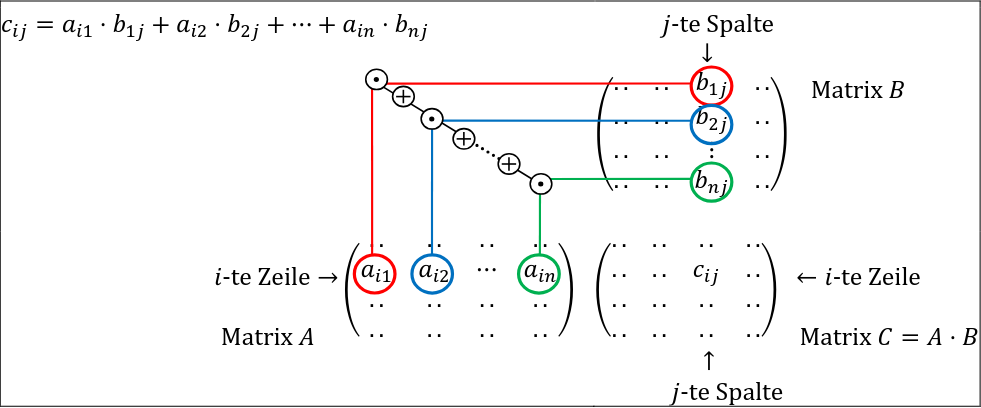
\includegraphics[scale=0.2]{images/matrixmult.png}
    \end{figure}
\end{minipage}
\hfill
\begin{minipage}[t]{0.45\textwidth}
    \subsubsection*{Transponierte Matrix}
    \begin{align*}
    A^T &= \begin{pmatrix}
    1 & 4 & 7 \\
    2 & 5 & 8 \\
    3 & 6 & 9
    \end{pmatrix}
    \end{align*}

    \subsubsection*{Multiplikation mit Skalar}
    \begin{align*}
    cA &= 2 \cdot A = \begin{pmatrix}
    2 & 4 & 6 \\
    8 & 10 & 12 \\
    14 & 16 & 18
    \end{pmatrix}
    \end{align*}
\end{minipage}

\section*{Lineare Gleichungssysteme}
\begin{minipage}[t]{0.45\textwidth}
    \subsection*{Zeilenstufenform}
    Die Matrix ist in Zeilenstufenform, wenn:
    \begin{itemize}
        \item Alle Zeilen, die nur Nullen enthalten, stehen am Ende der Matrix.
        \item Die erste Nicht-Null-Zahl in jeder Zeile (der sogenannte Pivot) ist 1 (führende Eins).
        \item Der Pivot jeder Zeile steht weiter rechts als der Pivot der vorherigen Zeile.
    \end{itemize}
    Reduzierte Zeilenstufenform (RREF) ist erreicht, wenn:
    \begin{itemize}
        \item Jede Spalte, die eine führende Eins enthält, hat nur Nullen in allen anderen Zeilen.
    \end{itemize}    
\end{minipage}
\hfill
\begin{minipage}[t]{0.45\textwidth}
    \subsection*{Parameterdarstellung}
    \subsubsection*{führende Unbekannte}
    Die führenden Unbekannten sind die Variablen, die in der Zeilenstufenform der Matrix als Pivot-Elemente auftreten. Sie sind eindeutig bestimmt und können direkt aus den Gleichungen abgelesen werden.
    \subsubsection*{freie Unbekannte}
    Die freien Unbekannten sind die Variablen, die nicht als Pivot-Elemente auftreten. Sie können beliebige Werte annehmen.
    
\end{minipage}
\subsubsection*{Beispiel}
\begin{align*}
    \begin{pmatrix}
    1 & -2 & 0 & 3 | 5 \\
    0 & 0 & 1 & 1 | 3
    \end{pmatrix}
\end{align*}
In diesem Beispiel sind $x_1$ und $x_3$ die führenden Unbekannten, während $x_2$ und $x_34$ freie Unbekannte sind. Die Lösung kann in Parameterform dargestellt werden:

\begin{minipage}[t]{0.45\textwidth}
    \begin{align*}
        x_2 &= \lambda \quad (\lambda \in \mathbb{R}) \\
        x_4 &= \mu \quad (\mu \in \mathbb{R})
    \end{align*}
    Erste Zeile: \( x_1 - 2x_2 + 3x_4 = 5 \), daraus \( x_1 = 5 + 2\lambda - 3\mu \)\\
    Zweite Zeile: \( x_3 + x_4 = 3 \), daraus \( x_3 = 3 - \mu \)
\end{minipage}
\hfill
\begin{minipage}[t]{0.45\textwidth}
    In Vektorform:

    \begin{align*}
        \begin{pmatrix}
        x_1 \\
        x_2 \\
        x_3 \\
        x_4
        \end{pmatrix}
        = 
        \begin{pmatrix}
        5 \\
        0 \\
        3 \\
        0
        \end{pmatrix}
        + \lambda
        \begin{pmatrix}
        2 \\
        1 \\
        0 \\
        0
        \end{pmatrix}
        + \mu
        \begin{pmatrix}
            -3 \\
            0 \\
            -1 \\
            1
        \end{pmatrix}
    \end{align*}
\end{minipage}

\section*{Lösbarkeit von LGS}
\begin{itemize}
    \item \textbf{Eindeutige Lösung:} Wenn die Matrix in Zeilenstufenform keine freien Unbekannten hat.
    \item \textbf{Unendlich viele Lösungen:} Wenn die Matrix in Zeilenstufenform mindestens eine freie Unbekannte hat.
    \item \textbf{Keine Lösung:} Wenn die Matrix in Zeilenstufenform eine Zeile der Form \(0 = c\) (mit \(c \neq 0\)) enthält.
\end{itemize}
\end{document}